\section{Theoretical Analysis}
\label{sec:analysis}

In this section we analyse the architecture chosen for the ACDC converter circuit using an Octave theoretical model. Using the ideal diode model we were able to predict the output of the Envelope Detector and using the incremental diode model we predicted the output of the Voltage Regulator.

\subsection{Envelope Detector}
Our input for the envelope detector is the AC voltage source with its amplitude reduced by the transformer. This voltage is processed by the full-wave bridge rectifier, which allows current to flow in both directions, unlike the half-wave rectifier, which only allows current to pass when our voltage source is at a positive state (otherwise the diode would be shut-off). The full-wave rectifier allows two possible paths for the current to flow, one for positive voltage, the other for negative voltage. This way, in $R_{env}$ the voltage will always be positive or nule, obviously mantaining its amplitude and frequency traits, since we are using the ideal diode model - no voltage is consummed by the diodes. The junction of the capacitor will annihilate the wave status of the voltage. When the voltage is at its peak, it will then start its periodic decrease, and the current in the capacitor will grow more and more negative until it reaches the point where its simmetric to the current flowing in the resistor! It's simple to see, using the nodal method, that the current flowing from the diode path is now null, and those diodes will shut-off. This happens, as stated, when $i_{R}$ = $i_{C}$, and the equation for the instant is given by:
\begin{equation}
t_{off} = \frac{1}{w} * arctan(\frac{1}{wRC});
\end{equation}
Now the capacitor will discharge through the resistor, and our output for the envelope detector will decay (remember that until $t_{off}$ our output voltage was equal to the one that comes out of the full-wave rectifier, the output voltage in the load (the resistor), which is the same voltage of the capacitor (since they're in paralell), which is then finally our envelope detector output voltage). The decay of our output voltage is expressed by the following equation, where $A$ is the amplitude of the input voltage, $\frac{230}{N_{coils}}$:
\begin{equation}
V_{env} = A|cos(wt_{off})|e^\frac{-(t-t_{off})}{RC};
\end{equation}
When the full-wave voltage becomes once again greater than our decay voltage (which is due to happen since it will reach the amplitude peak again and the voltage in the RC circuit is ever diminuishing). There, our envelope detector output voltage returns to being the one that comes out of the rectifier. Eventually, the rectifier voltage reaches its peak again (which happens a half of a period after - we're considering the negative peaks as well, which are now positive fruit of the rectifier's action) and the cycle repeats

Due to the transition regime we found in the NGSpice simulation, as you will see, that turned out to be quite lengthy, we opted to start the study of the circuit after a period of 3.8 seconds in order to have a stabilized response.
The voltage at the output of the envelope detector circuit is now plotted as follows in figure~\ref{fig:enveloped}.
\begin{figure}[h!] \centering
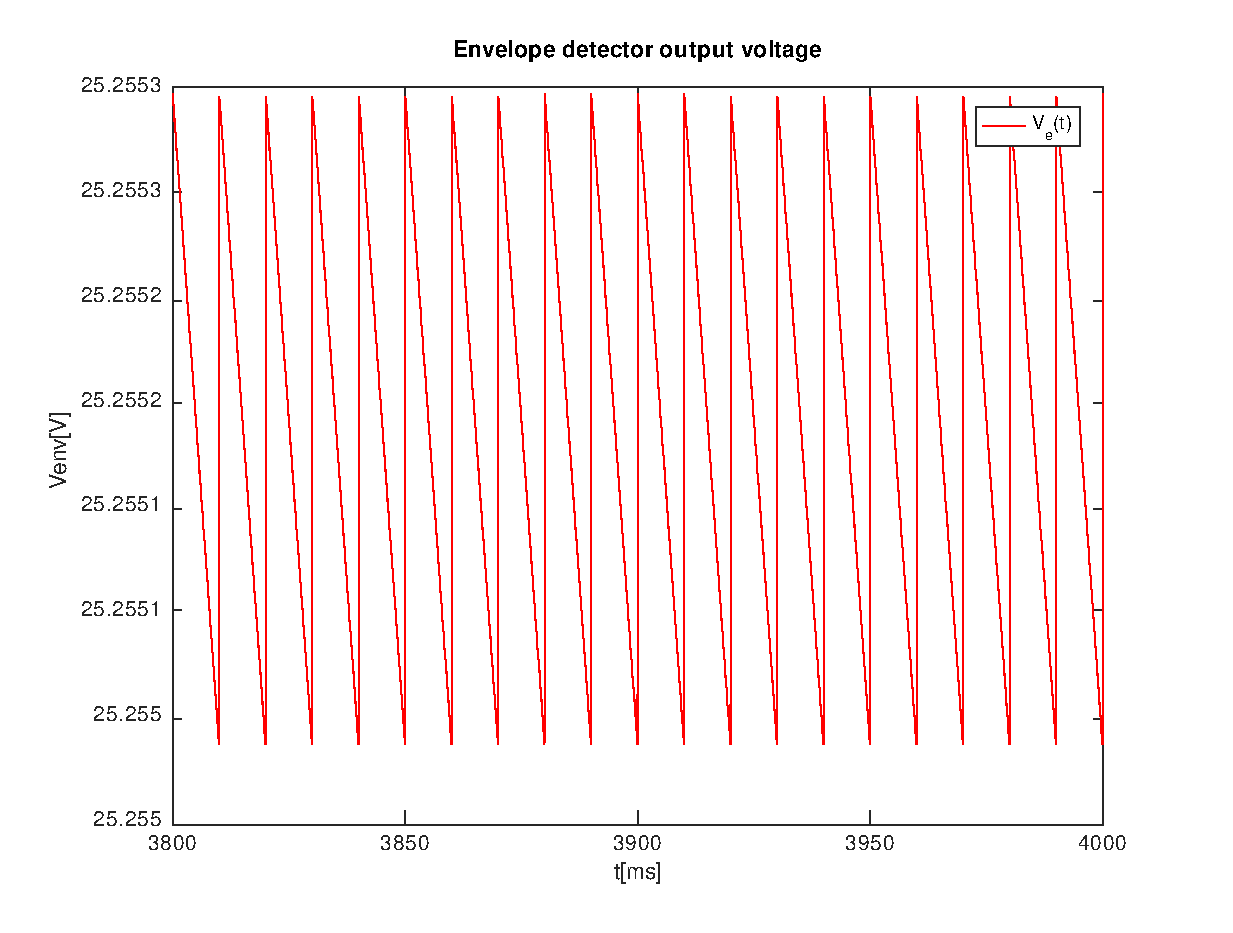
\includegraphics[width=0.6\linewidth]{Venv.eps}
\caption{Voltage envelope detector circuit output.}
\label{fig:enveloped}
\end{figure} \par
As expected, we see a positive voltage oscillating up to a maximum voltage equal to the initial 230V divided by the number of coils $\cong$ 25.2553V. Already we are close to a direct current regime, but the voltage level and the magnitude of the ripple still need to be addressed and adjusted. In table~\ref{tab:envio}, we present the average (DC component) and the ripple (the oscillation, the AC character) of the output from the envelope detector, which will now be our input voltage for our next step - the voltage regulator.

\begin{table}[h]
  \centering
  \begin{tabular}{|l|r|}
    \hline    
    {\bf Name} & {\bf Values [V]} \\ \hline
    \input{envelope_tab} 
  \end{tabular}
  \caption{Envelope Detector Output Voltage traits.}
  \label{tab:envio}
\end{table}

\subsection{Voltage Regulator}
For the voltage regulator, we used the incremental model. In the previous subsection, we divided our new input voltage in its DC and AC component, and we will now treat them separately. Starting with the DC component, for this step the ideal model with a voltage source $V_{ON}$ is used. We chose $V_{ON} = 0.6$, in accordance to our number of diodes, 20, so that our final output voltage, the output in the series of diodes, is the desired 12V. So, if our input DC voltage is greater than 12V, the current will flow and our DC output voltage will be 12V - since our input DC component is purposely greater than 12V, then our DC component for the voltage regulator is guaranteed to be 12V.
For the AC component, every diode is represented by a resistor, $r_d$, whose resistance can be calculated according to the following formula:
\begin{equation}
r_d=\frac{\eta*V_T}{I_S*e^\frac{V_D}{\eta*V_T}}=~247.05;
\end{equation}
$I_{S}$ is the reverse saturation current, with a value of $10^{-14}$, $\eta$ is the material constant, valued 1, and $V_{T}$ is the thermal voltage, with a value of $26 mV$ - all this values are the default values used by NGSpice for the default diode model. $V_D$ is the DC voltage in each diode - $V_{ON}$. This being said, our circuit is now equivalent to a voltage divider circuit, with the greater resistante, $R_{reg}$ and the sum of the diode resistances $r_d$ making up our output, so our AC output voltage can then be calculated in each time instance by the this next formula:
\begin{equation}
v_o = \frac{20r_d}{R + 20r_d}v_{env};
\end{equation}
This way, we needed a resistance value much greater than the diode incremental resistance (we chose 100kOhm) in order to diminuish our AC output voltage. This AC component is the inevitable variation of our output voltage around the 12V - the ripple - fruit of the sinusoidal character of our input voltage that can never be trully extinguished. Finally, our voltage regulator output and so our final output voltage consists of the adding effect of both the DC and AC components. 
The output of the regulator circuit is plotted in figures \ref{fig:reg} to \ref{fig:output}. In table~\ref{tab:regula} we can see the DC component and ripple of our final output, as well as the figure of merit such results would give us. However, the figure of merit desired is the one obtained in the simulation.
\begin{figure}[h!] \centering
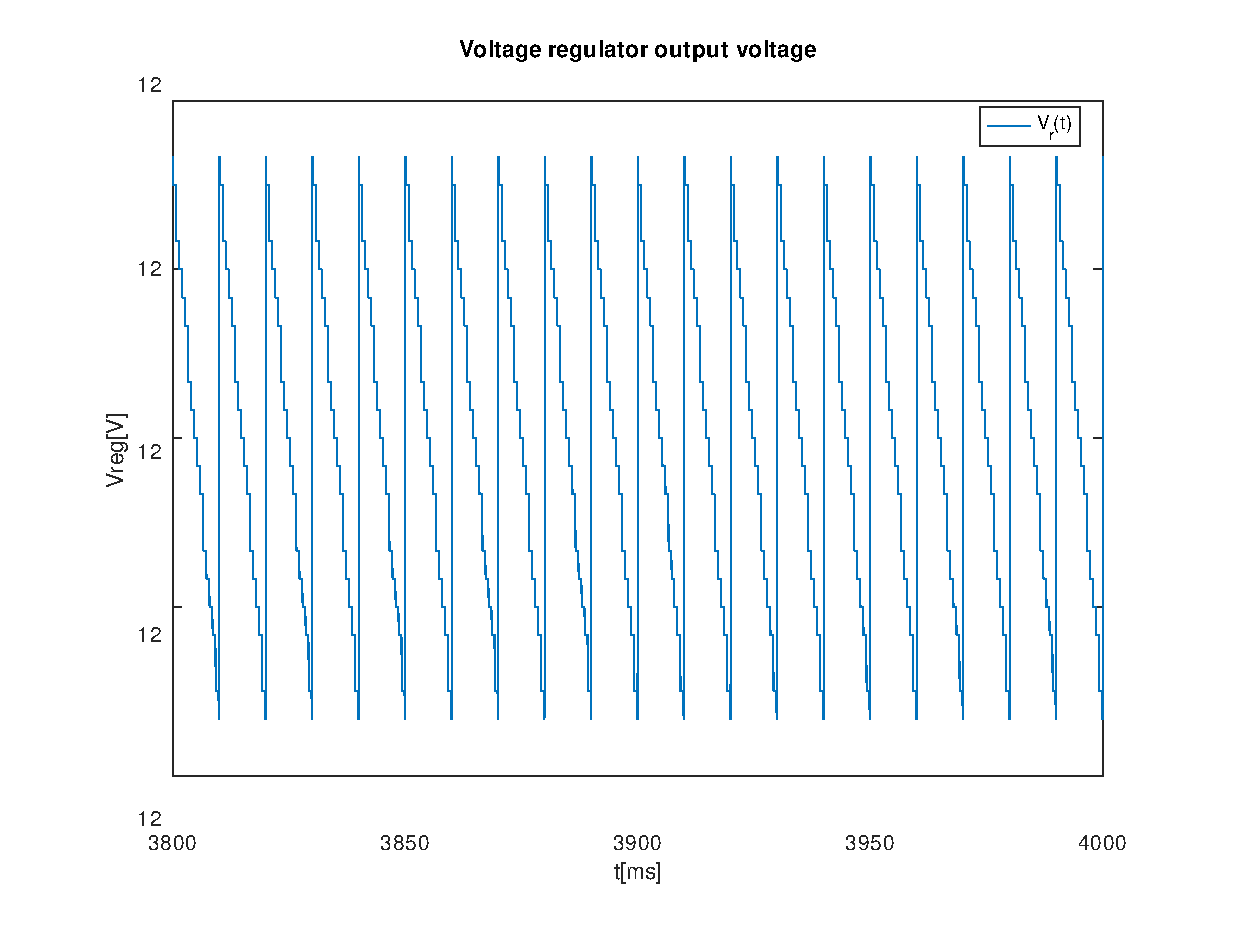
\includegraphics[width=0.6\linewidth]{Vreg.eps}
\caption{Voltage regulator circuit output.}
\label{fig:reg}
\end{figure}
\begin{figure}[h!] \centering
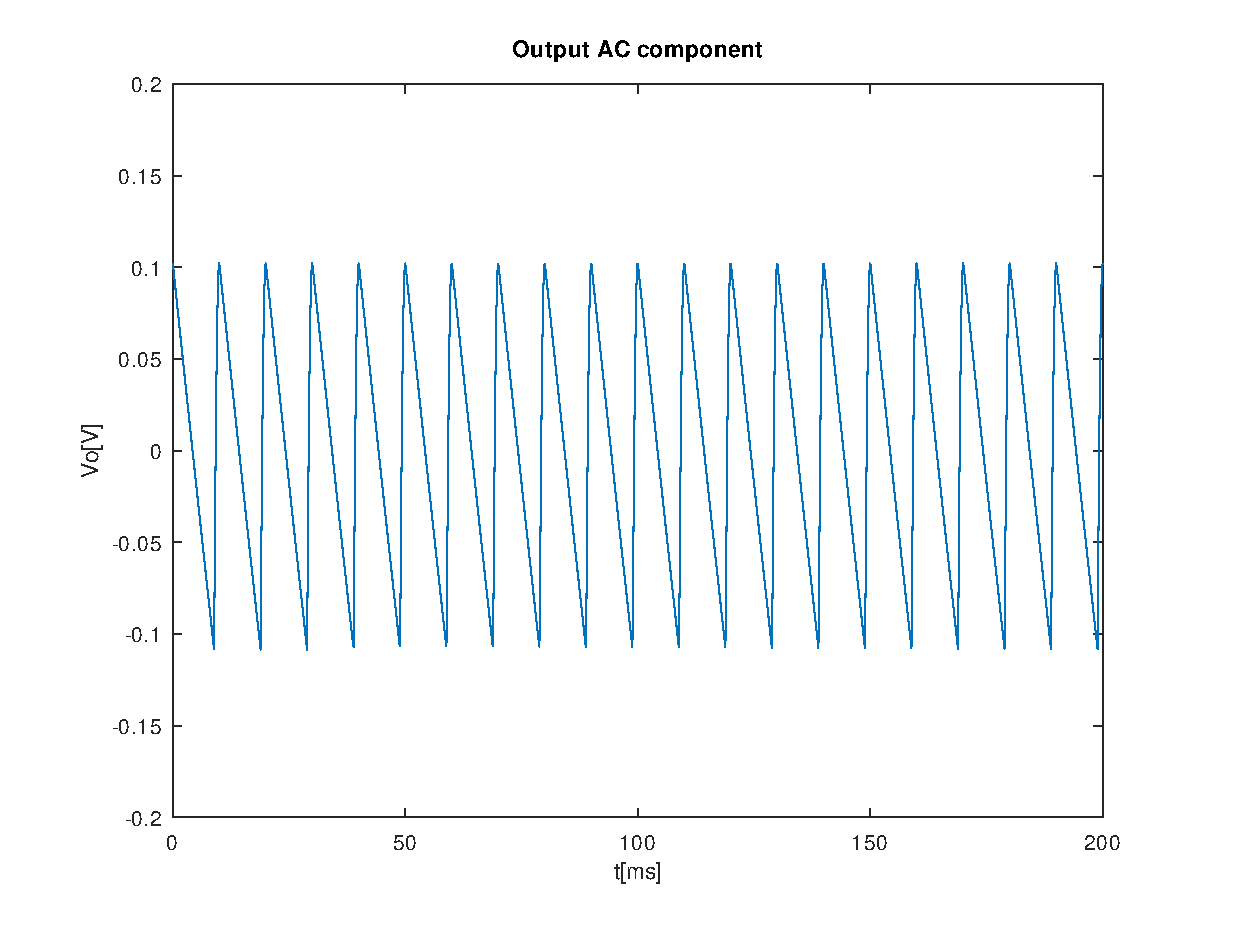
\includegraphics[width=0.6\linewidth]{deviation.eps}
\caption{Circuit output subtracted of the desired 12V.}
\label{fig:dc}
\end{figure}

\begin{table}[h]
  \centering
  \begin{tabular}{|l|r|}
    \hline    
    {\bf Name} & {\bf Values [V]} \\ \hline
    @$V_{DC}$ & 12.000000 \\ \hline 
@$V_{ACripple}$ & 0.000015 \\ \hline 
Cost & 1902.400000 \\ \hline 
Merit & 33.573648 \\ \hline 
 
  \end{tabular}
  \caption{Voltage Regulator Output Voltage traits, and theoretical figure of merit.}
  \label{tab:regula}
\end{table}
As we can see in this table, the ripple is very low, in an order of greatness of the uV (15 uV), which is a very much pleasing result to be replicated in the simulation.

\begin{figure}[h!] \centering
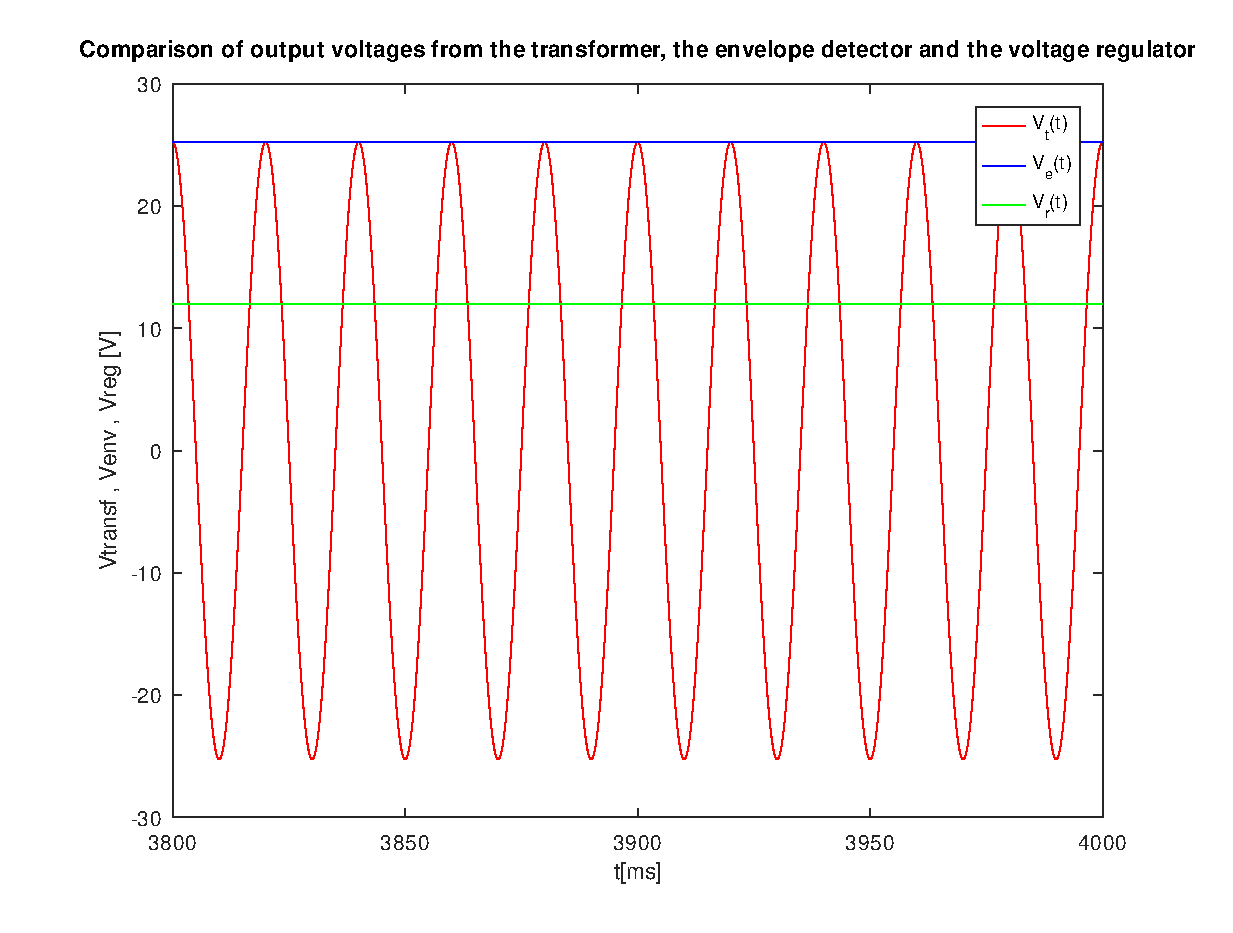
\includegraphics[width=0.75\linewidth]{comparison.eps}
\caption{Comparison between the different voltage outputs.}
\label{fig:output}
\end{figure}
\par
